\documentclass[border=10pt]{standalone}

\usepackage{tikz}
\usepackage{tikzsymbols}
\usetikzlibrary{calc,patterns,shapes.geometric}

\def\centerarc[#1](#2)(#3:#4:#5){\draw[#1] ($(#2)+({#5*cos(#3)},{#5*sin(#3)})$) arc (#3:#4:#5);}

\begin{document}
	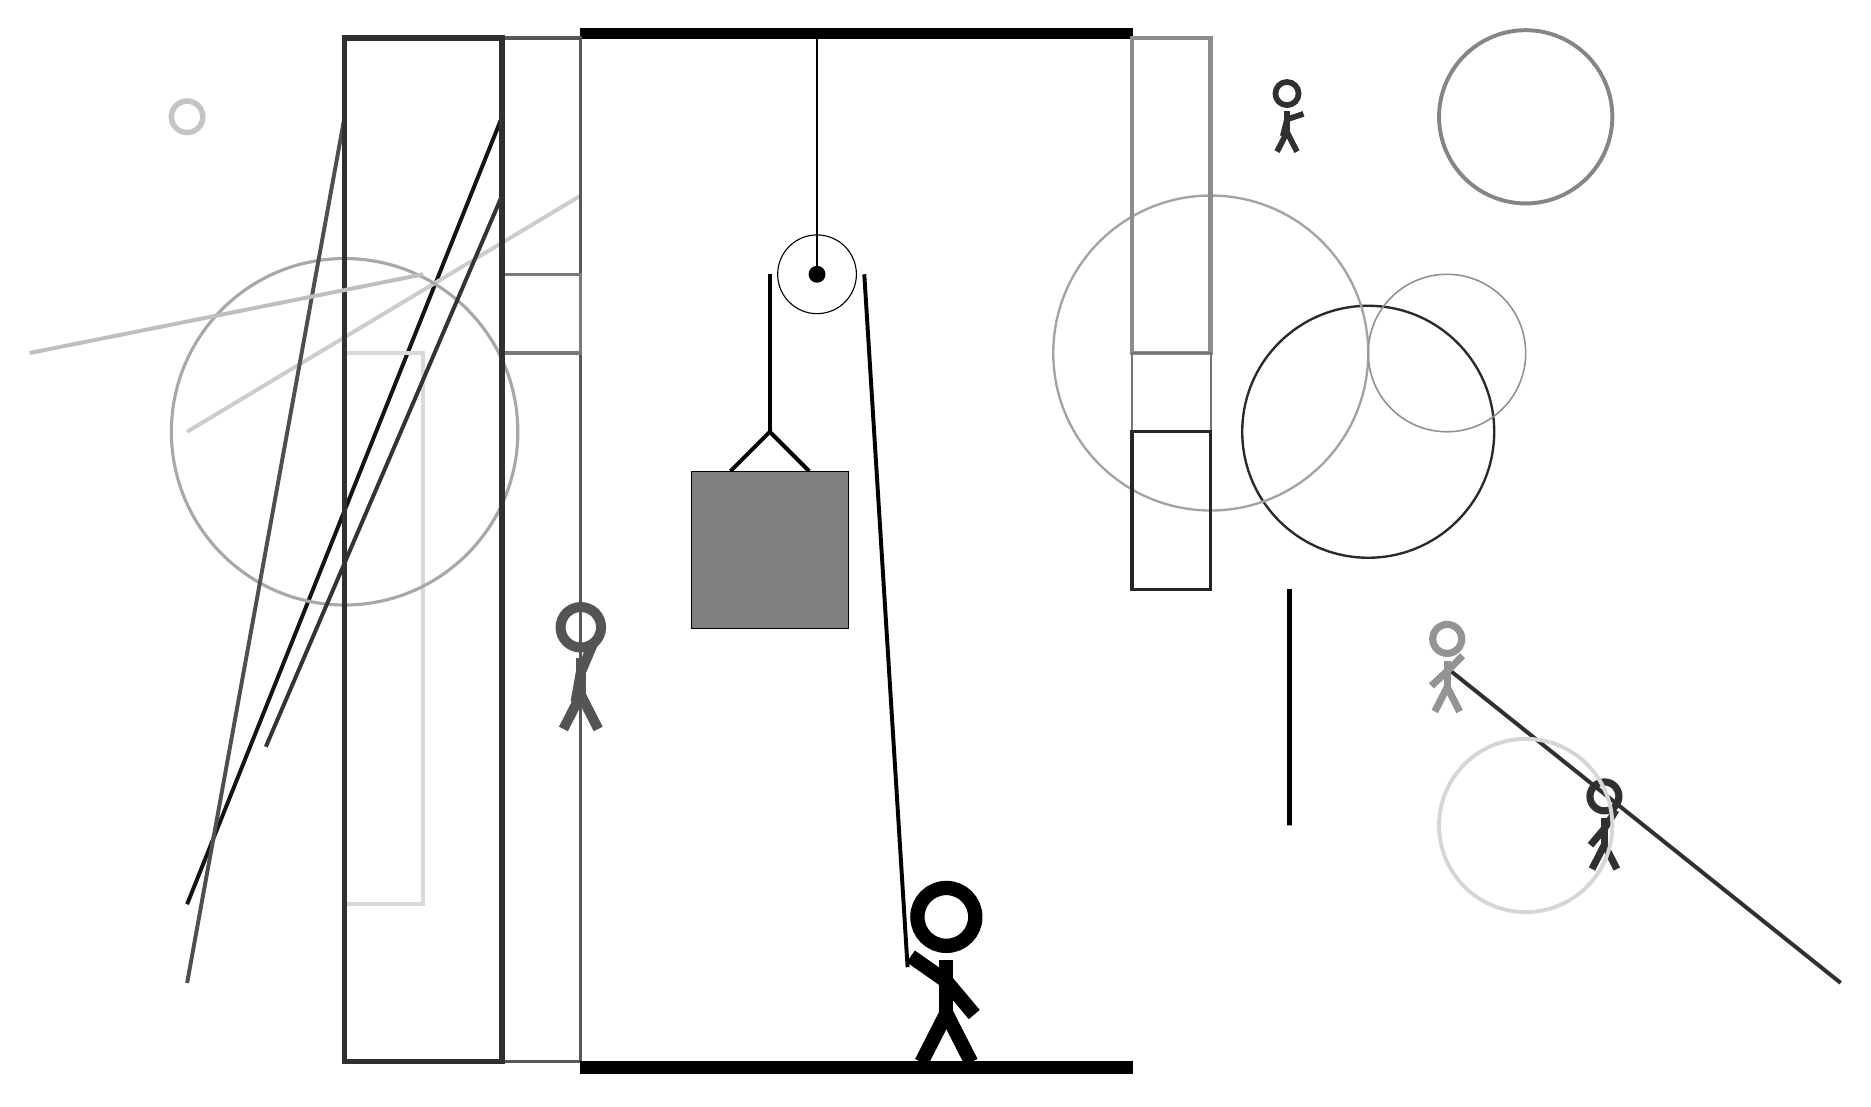
\begin{tikzpicture}
		%%%%% START %%%%%
		
		\draw[fill=black] (-2, 10) rectangle (5, 10.125);
		
		\draw (1, 7) circle (0.5);
		\draw[fill=black] (1, 7) circle (0.1);
		\draw (1, 10) -- (1, 7);
		
		\draw[line width=0.5mm] (-0.1, 4.5) -- (0.4, 5.0) -- (0.9, 4.5);
		\draw[fill=black!50] (-0.6, 4.5) rectangle (1.4, 2.5);
		
		\draw [line width=0.5mm, color=black!48](10, 9) circle (1.1);
		
		\draw[line width=0.5mm, color=black!92](-3, 9) -- (-7, -1);
		\draw[line width=0.5mm, color=black!81](9, 2) -- (14, -2);
		\draw [line width=0.3mm, color=black!84](8, 5) circle (1.6);
		\draw [line width=0.3mm, color=black!36](6, 6) circle (2.0);
		\draw[line width=0.6mm, color=black!45] (6, 10) rectangle (5, 6);
		
		\draw[line width=0.5mm, color=black!20](-7, 5) -- (-2, 8);
		
		\draw[line width=0.6mm, color=black!100] (7, 0) rectangle (7, 3);
		\draw[line width=0.5mm, color=black!15] (-4, -1) rectangle (-5, 6);
		
		\draw [line width=0.2mm, color=black!43](9, 6) circle (1.0);
		
		\draw[line width=0.4mm, color=black!66] (-3, 10) rectangle (-2, -3);
		\draw [line width=0.4mm, color=black!34](-5, 5) circle (2.2);
		\draw[line width=0.5mm, color=black!69](-5, 9) -- (-7, -2);
		
		\draw[line width=0.5mm, color=black!100](-3, 2) -- (-3, 5);
		\draw[line width=0.4mm, color=black!52] (-3, 7) rectangle (-2, 6);
		\node[line width=0.6mm, color=black!81] at (11, 0) {\Strichmaxerl[5][50][58]};
		
		\node[line width=0.5mm, color=black!81] at (7, 9) {\Strichmaxerl[4][76][18]};
		\draw[line width=0.7mm, color=black!81] (-3, -3) rectangle (-5, 10);
		\draw[line width=0.5mm, color=black!25](-4, 7) -- (-9, 6);
		\draw [line width=0.7mm, color=black!23](-7, 9) circle (0.2);
		\node[line width=0.3mm, color=black!42] at (9, 2) {\Strichmaxerl[5][43][45]};
		
		\draw[line width=0.5mm, color=black!80](-3, 8) -- (-6, 1);
		
		\draw[line width=0.3mm, color=black!55] (6, 6) rectangle (5, 5);
		\draw[line width=0.4mm, color=black!85] (5, 3) rectangle (6, 5);
		\node[line width=0.6mm, color=black!67] at (-2, 2) {\Strichmaxerl[7][80][67]};
		\draw [line width=0.5mm, color=black!16](10, 0) circle (1.1);
		
		\draw[line width=0.5mm] (0.4, 7) -- (0.4, 5.0);
		\centerarc[line width=0.5mm](1, 7)(0:180:0.6);
		\draw[line width=0.5mm](1.6, 7) -- (2.15, -1.8);
		
		\node at (2.6, -1.9) {\Strichmaxerl[10][-35][-50]};
		
		\draw[fill=black] (-2, -3) rectangle (5, -3.15);
		
		%%%%% END %%%%%
	\end{tikzpicture}
\end{document}